\section*{Appendix}

\begin{figure}[H]
\begin{center}
   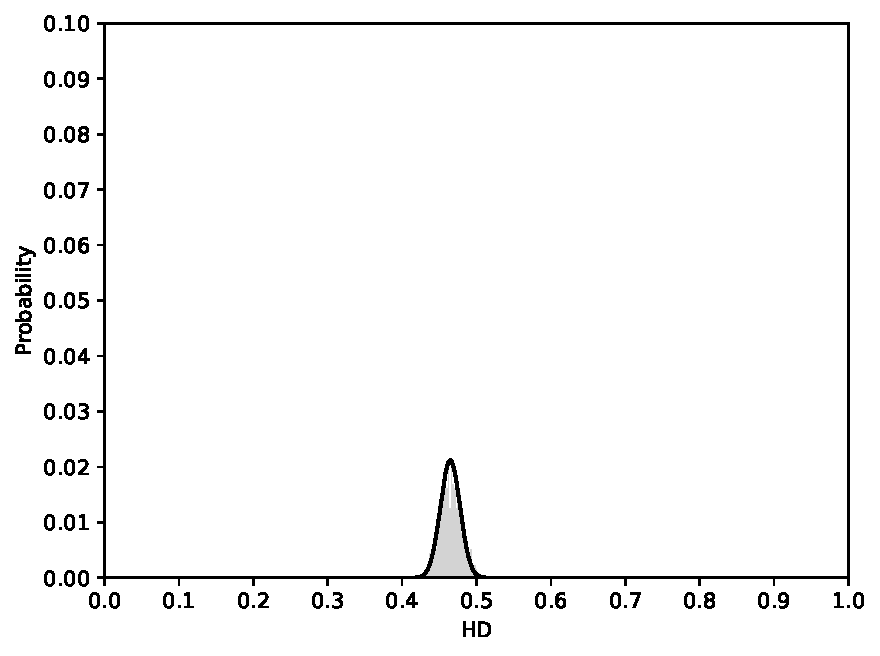
\includegraphics[scale=0.6]{HD_distribution2.pdf}
   \caption{Hamming distance distribution and the corresponding binomial distribution overlaid. Plot generated with~\cite{bob2017}. }
   \label{fig:binom}
\end{center}
\end{figure}


We explicitly state the data represented by the pair identifier $i=0 \dots 19$:
\begin{itemize}
    \item (0,  `5\_right\_middle\_1\_cam1.png',  `5\_right\_middle\_2\_cam1.png')
    \item (1,  `5\_right\_middle\_1\_cam2.png',  `5\_right\_middle\_2\_cam2.png')
    \item (2,  `5\_left\_ring\_1\_cam1.png',  `5\_left\_ring\_2\_cam1.png')
    \item (3,  `5\_right\_ring\_1\_cam1.png',  `5\_right\_ring\_2\_cam1.png')
    \item (4,  `5\_left\_ring\_1\_cam2.png',  `5\_left\_ring\_2\_cam2.png')
    \item (5,  `5\_right\_ring\_1\_cam2.png',  `5\_right\_ring\_2\_cam2.png')
    \item (6,  `5\_right\_index\_1\_cam1.png',  `5\_right\_index\_2\_cam1.png')
    \item (7,  `5\_right\_index\_1\_cam2.png',  `5\_right\_index\_2\_cam2.png')
    \item (8,  `3\_left\_middle\_1\_cam1.png',  `3\_left\_middle\_2\_cam1.png')
    \item (9,  `3\_right\_middle\_1\_cam1.png',  `3\_right\_middle\_2\_cam1.png')
    \item (10,  `3\_left\_middle\_1\_cam2.png',  `3\_left\_middle\_2\_cam2.png')
    \item (11,  `3\_right\_middle\_1\_cam2.png',  `3\_right\_middle\_2\_cam2.png')
    \item (12,  `3\_left\_ring\_1\_cam1.png',  `3\_left\_ring\_2\_cam1.png')
    \item (13,  `3\_right\_ring\_1\_cam1.png',  `3\_right\_ring\_2\_cam1.png')
    \item (14,  `3\_left\_ring\_1\_cam2.png',  `3\_left\_ring\_2\_cam2.png')
    \item (15,  `3\_right\_ring\_1\_cam2.png',  `3\_right\_ring\_2\_cam2.png')
    \item (16,  `3\_left\_index\_1\_cam1.png',  `3\_left\_index\_2\_cam1.png')
    \item (17,  `3\_right\_index\_1\_cam1.png',  `3\_right\_index\_2\_cam1.png')
    \item (18,  `3\_left\_index\_1\_cam2.png',  `3\_left\_index\_2\_cam2.png')
    \item (19,  `3\_right\_index\_1\_cam2.png',  `3\_right\_index\_2\_cam2.png')
\end{itemize}


